\section{Approach}
\label{sec:exploring-boundaries:Approach}
Our goal is to generate reliable code from models specified using a DSML.
To increase the reliability of generated code, formal methods such as verification can be used.
To ensure that the same model is verified and executed, models specified using the DSML should automatically be transformed to models suitable for these purposes.
In this way, these models do not have to be created by hand.
This enables the use of formal methods without having to create models suitable for that purpose separately.
This has the advantage that engineers do not have to learn the syntax and semantics of different languages.
Moreover, manual transformation is a slow and error-prone task.

Often, DSMLs and their envisaged implementation platforms have different semantical characteristics.
Therefore, the semantic gap between the two formalisms needs to be bridged~\cite{Amstel2008}.
We propose to use model transformations to refine DSML models in such a way that the semantic properties of the DSML and the implementation platform are aligned.
In this way, the abstract DSML model becomes concrete and transformation from the refined (concrete) model to executable code is merely a syntactical transformation.
%%%%%%%%%%%%%%%%%%%%%%%%%%%%%%%%%%%%%%%%%%%%%%%%%%%%%%%%%%%%%%%%%
%%% Leg uit hoe een DSML zowel abstract als concreet kan zijn  %%%
%%% Meerdere abstractieniveau's toegestaan                    %%%
%%%%%%%%%%%%%%%%%%%%%%%%%%%%%%%%%%%%%%%%%%%%%%%%%%%%%%%%%%%%%%%%%

To enable verification of DSML models, a transformation from the DSML to a formalism for verification should be implemented.
For our experiments, we implemented a transformation to a model checking formalism.
Using this transformation, it is possible to verify whether both the abstract and the concrete DSML models fulfill their requirements.
From the experiments presented in Section~\ref{sec:exploring-boundaries:Experiments}, we concluded that verification of an abstract model poses no problems.
However, verification of a concrete model is infeasible because the verification takes too much time and needs too many resources.

The sequences of transformations used to refine the abstract DSML models produce intermediate models.
These models can be transformed to a verification formalism too.
By verifying the intermediate models, it is possible to verify models that are more concrete.
This approach is schematically depicted in the top half of Figure~\ref{fig:exploring-boundaries:mc_approach}.
The check marks indicate models that can be verified, whereas the crosses indicate models that cannot be verified.
\begin{figure}[hbt]
 \centering
 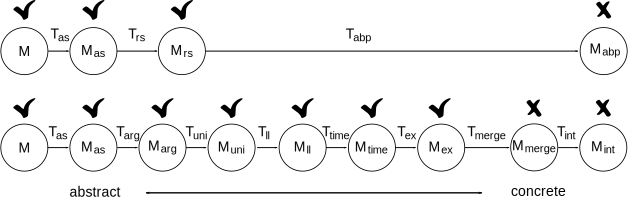
\includegraphics[width=.7\columnwidth]{exploring-boundaries/figs/fine-grained-transformations}
 \caption{Verification of intermediate models}
 \label{fig:exploring-boundaries:mc_approach}
\end{figure}
Our experiments showed that it is possible to verify some of the intermediate models, but the most concrete model that can be verified contains little implementation details.
Because the change induced on the models by the transformations is too large, the intermediate models suffer from state-space explosion after only a few refinement steps.
Therefore, we propose to use more fine-grained sequences of transformations to enable verification of more concrete models.
This can be achieved by splitting existing transformations into smaller parts.
In this way, more intermediate models are generated that can be verified.
This approach is schematically depicted in the bottom half of Figure~\ref{fig:exploring-boundaries:mc_approach}.
Using this approach, it is possible to verify models that are closer to the concrete model.
By replacing the transformations~\Transformation{rs} and~\Transformation{abp} from Figure~\ref{fig:exploring-boundaries:mc_approach} by the smaller transformations~\Transformation{arg}, \Transformation{uni}, \Transformation{ll}, \Transformation{time}, \Transformation{ex}, \Transformation{merge}, and~\Transformation{int}, for instance, the state space of the intermediate model~\Model{ex} can be explored, instead of that of the less concrete model~\Model{rs}.
The example shown in Figure~\ref{fig:exploring-boundaries:mc_approach} is an illustration of one of the experiments presented in Section~\ref{sec:exploring-boundaries:Experiments}.
In different cases, the transformation steps as well as which intermediate models can be verified will vary.

The most concrete model that can be model checked may still not be close enough to the implementation model.
An attempt can be made to split the transformations into even smaller parts.
If this is not possible anymore, another possibility is to apply the model transformation to part of the model only.
Since the refinement, in this case, is applied to a small part of the model, this will most likely result in models that give rise to smaller state spaces.
Using partial refinement, the boundaries of what can be verified using model checking can be explored even further.

Using more fine-grained sequences of transformations has some positive side-effects.
Since the individual transformations of fine-grained sequences of transformations tend to be smaller than those of course-grained ones, it is easier to locate defects in them.
Additionally, these transformations have proven to be more reusable than those used to form course-grained sequences during our experiments.
Another advantage of having fine-grained sequences of transformations is that it enables shuffling the order in which the transformations are applied.
This order affects the output model, however, and some sequences of transformations may lead to more efficient implementations than others.
Furthermore, it may be that not all orderings are allowed because the preconditions of some transformations may be in conflict with the postcondition of others. 